%% LaTeX2e class for student theses
%% sections/evaluation.tex
%% 
%% Karlsruhe Institute of Technology
%% Institute for Program Structures and Data Organization
%% Chair for Software Design and Quality (SDQ)
%%
%% Dr.-Ing. Erik Burger
%% burger@kit.edu
%%
%% Version 1.3.6, 2022-09-28

\chapter{Related Work}
\label{ch:Related_work}
Related work for this thesis can be grouped into three different categories: The first category is \hyperref[sec:Related_work:Active_Learning]
{Active Learning}. Active Learning is a special form of machine learning where an oracle is present which can label arbitrary data points.
A Machine Learning model trained using Active Learning iteratively queries the oracle with unlabeled data points, trains a new model and
determines which data should be queried next. The second category is \hyperref[sec:Related_work:Continual_Learning]{Continual Learning}.
Continual learning is a machine learning technique which aims to make a given machine learning model learn new tasks without forgetting
the knowledge of previous tasks. The third category is \hyperref[sec:Related_work:Model_Stealing]{Model Stealing}. Model Stealing is the process
of strategically querying a third-party machine learning model (also referred to as target model) to train a local model (also referred to as
substitute model) which is supposed to approximate the target model as good as possible. These three categories have been covered in chapter
\ref{ch:Background} in more detail. In this chapter, we will focus on the specific approaches from these three research directions which
are either used in the experiments of this thesis or are related to the approaches used in the experiments.

% use Settles as reference for the general introduction
% Mention that active learning is a specific form of semi-supervised learning (according to Mundt et al.)
\section{Active Learning}
\label{sec:Related_work:Active_Learning}
\subsection{General Introduction}
Active Learning is a specific form of machine learning where the learner can query an oracle to label arbitrary data points.
The motivation behind Active Learning is that nowadays it is not difficult to obtain large amounts of data, but the bottleneck
is assigning labels to them. Active Learning aims to overcome this issue by producing a highly accurate model with little amount
 of labeled data. The idea is that a learner which chooses the data it is trained on should perform better or at least as good
 as a model trained on all available data.
\subsection{Active Learning Approaches used in the Experiments}
\label{sec:Related_work:Active_Learning:Approaches}
\subsubsection{Least Confidence}
Least Confidence (LC) is one of the earlier and simpler approaches to Active Learning. LC is an uncertainty-based Active Learning
approach proposed by Lewis et al. \cite{lewis1994sequential} in 1994. The idea behind LC is that the next points to label should be the 
ones with the lowest prediction probability. More formally, the data queried will be the following:
\begin{equation}
    \argmin_{x \in \mathcal{U}} \max_{y \in \mathcal{Y}} p(y|x)
\end{equation}
\subsubsection{CoreSet}
CoreSet, sometimes also referred to as k-center strategy, is an Active Learning approach specifically proposed for Convolutional Neural
Networks \cite{sener2017active}. Sener \& Savarese redefine the pool-based Active Learning problem (for original definition see \ref{sec:PoolBasedActiveLearning})
as 
\begin{equation}
    \min_{s^1 \subseteq U: |s^1| \leq b } \abs{\frac{1}{|L \cup U|} \sum_{x_i,y_i \in L \cup U} l(x_i,y_i;L \cup s^1) - \frac{1}{|L \cup s^1|} \sum_{j \in L \cup s^1} l(x_j,y_j,L \cup s^1)} 
\end{equation}
Informally, this can be seen as selecting the data points to add to the labeled pool which ensure best the best loss approximation of a model trained on the labeled set compared
to a model trained on the whole dataset. The authors assume zero training error, which simplifies the equation above to
\begin{equation}
    \frac{1}{|L \cup U|} \sum_{x_i,y_i \in L \cup U} l(x_i,y_i;L \cup s^1)
\end{equation}
Sener \& Savarese show that minimizing this equation is equivalent to solving the k-Center problem \cite{wolf2011facility}, i.e.
\begin{equation}
    \min_{s^1: |s^1| \leq b} \max_i \min_{j \in s^1 \cup L}  \Delta (x_i,x_j)
\end{equation}
This problem is NP-Hard but can be solved by a 2-OPT Greedy Algorithm.
\begin{algorithm}
    \caption{k-Center-Greedy} \label{alg:kCenterGreedy}
    \begin{algorithmic}
        \Require data $x_i$, labeled pool $L$ and budget $b$
        \State Initialize s = $L$
        \Repeat
        \State $u = \argmax_{x_i \in U \setminus s} \min_{x_j \in s} \Delta(x_i,x_j)$
        \State $s = s \cup \{u\}$
        \Until{$|s| = b$}
        \return $s \setminus L$
    \end{algorithmic}
\end{algorithm}
The authors propose a more sophisticated algorithm which performs marginally better than the greedy solution but is approximately 4 times slower. We therefore omit the proposed algorithm in this 
section.
% Talk about distance metric used here.
\subsubsection{BALD}
% Hier noch Monte Carlo Dropout von Gal et al. erwähnen (2017)
Bayesian Active Learning by Disagreement (BALD) is an uncertainty-based Active Learning Strategy proposed by Houlsby et al. \cite{houlsby2011bayesian}. BALD uses Shannon's entropy \cite{cover1991information}
to determine a model's prediction uncertainty for a given unlabeled data point. More precisely, a learner using  BALD will query the sample(s) fulfilling the following condition:
\begin{equation}
    \argmax_x H[y \mid x, L] - \mathbb{E}_{\theta \sim p(\theta \mid L)} [H[y \mid x, \theta]]
\end{equation}
Informally, BALD selects those data points with the biggest gap between the model's actual prediction uncertainty and the model's expected prediction uncertainty. Since the expected prediction uncertainty cannot
be computed given that the parameter distribution conditioned on the previously observed data is unknown, BALD uses Monte Carlo sampling to approximate the expected prediction uncertainty. For neural networks, Monte
Carlo Dropout \cite{gal2016dropout} can be applied.
\subsubsection{Badge}
Batch Active Learning by Diverse Gradient Embeddings (Badge) \cite{ash2019deep} is a Batch Active Learning strategy which combines both model uncertainty and batch-diversity to select the next batch of data points
to label. The authors were inspired to develop Badge by the observation that diversity-based Active Learning strategies perform well in the first few iterations diversity-based approaches perform well while in the
later stages of Active Learning uncertainty-based approaches perform well. Badge therefore incorporates both uncertainty and diversity in its selection strategy. Badge uses the gradient with respect to the output
layer as a measure of model uncertainty, similar to the ideas of \cite{zhang2017active} and \cite{settles2007multiple}. Since Badge works on unlabeled data points, the gradient cannot be computed exactly because
the label is unknown. Therefore, Badge uses the hypothetical label $\hat{y}(x)$ as a proxy for the true label and computes the gradient of the cross-entropy loss on the hypothetical label as an approximation of the
real gradient. To incorporate diversity, Badge uses $k$-means++ clustering \cite{arthur2007k} for the gradient embeddings to sample the next batch of data points to label. The authors demonstrate Badge's agnosticism
towards model architecture, training hyperparameters and dataset in a variety of experiments. 
\begin{algorithm}
    \caption{BADGE} \label{alg:Badge}
    \begin{algorithmic}[1]
        \Require Neural network $f(x;\theta)$, unlabeled pool $U$, labeled pool $L=\emptyset$, number of iterations $T$, bath size $b$
        \State Labeled dataset $L \leftarrow k$ random samples from $U$ together with their labels
        \State Train initial model $\theta_1$ on $L$
        \For{$t = 1,2,\ldots,T$}
            \State For all examples $x$ in $U \setminus L$:
            \begin{enumerate}[leftmargin=0.8in]
                \item Compute its hypothetical label $\hat{y}(x) = h_{\theta_t}(x)$
                \item Compute gradient embeddings $g_x = \frac{\partial}{\partial \theta_{out}} l_{\text{CE}}(f(x;\theta_t),\hat{y}(x))$, where $\theta_{out}$ refers to
                parameters of the final (output) layer.
            \end{enumerate}
            \State Compute $S_t$, a subset of $U \setminus L$ of size $b$, using the $k$-MEANS++ seeding algorithm on {\color{white} 123}$\{ g_x: x \in U \setminus L\}$ and query for
            their labels.
            \State Update labeled pool $L \leftarrow L \cup S_t$
            \State Train new model $\theta_{t+1}$ on $L$
        \EndFor
        \return Final model $\theta_T$
    \end{algorithmic}
\end{algorithm}
% Structure: First some general introduction then present
% the different approaches used in the experiments (LC, CoreSet, BALD, Badge)

% Use parisi et al. as reference for the general introduction
% Synaptic Intelligence paper also gives good introduction into approaches and structures them
% into three categories
% Also mention the difference between task-incremental, class-incremental and domain-incremental learning
\section{Continual Learning}
\label{sec:Related_work:Continual_Learning}
\subsection{General Introduction}
Artificial Neural Networks suffer from a problem called \enquote{Catastrophic Forgetting} \cite{mccloskey1989catastrophic}.
Catastrophic Forgetting is the phenomenon that the performance of a neural network previously trained on task $t_{n-k}$
severely decreases when the same neural network is later trained on task $t_n (k>0)$. More briefly, neural networks struggle
to retain the knowledge of previous tasks when learning new tasks. The problem of Catastrophic Forgetting has wide-ranging
implications for the use of neural networks because it limits their use to settings where the data at deployment time is
distributed identically to the data observed at training time. Clearly, this is not the case in most real-world applications.
Research in Continual Learning aims to develop mechanisms which alleviate Catastrophic Forgetting. The Continual Learning approaches
which have been proposed so far can be grouped into three categories according to \cite{mundt2020wholistic} and
\cite{zenke2017continual}. Mundt et al. \cite{mundt2020wholistic} propose to group Continual Learning approaches into
\textbf{regularization}, \textbf{rehearsal} and \textbf{architectural} approaches whereas Zenke et al. \cite{zenke2017continual}
group Continual Learning approaches into \textbf{architectural},\textbf{functional} and \textbf{structural} approaches. In the
following, we will stick to the categorization proposed by Mundt et al. because it is broader and fully encompasses the
categorization by Zenke et al.
\subsubsection{Regularization}
Regularization-based approaches to Continual Learning aim to prevent the forgetting of previous tasks by adding a regularization
term to the model's loss function. The regularization term is used as a proxy for how much the performance of the model on previous
tasks will decrease, i.e. a high regularization term indicates that the model will perform poorly on the old tasks with the current
weights and a low regularization term indicates that the model has not lost much knowledge of the old tasks. The way the
regularization term is computed can further be divided into two groups. There are \textbf{structural} approaches which regularize
based on weight changes to the model and there are \textbf{functional} approaches which regularize based on the output of the model.
Notable examples of structural approaches include Elastic Weight Consolidation (EWC) \cite{kirkpatrick2017overcoming},Memory Aware
Synapses (MAS) \cite{aljundi2018memory}, Incremental Moment Matching (IMM) \cite{lee2017overcoming} as well as Asymmetric Loss
Approximation by Single-Side Overestimation (ALASSO) \cite{park2019continual} which is an extension of Synaptic Intelligence (SI)
\cite{zenke2017continual}. All the structural regularization approaches will be covered in more detail in the section on
\hyperref[sec:Related_work:Continual_Learning:Experiments]{the continual learning approaches used in the experiments}. \\
Functional regularization approaches are inspired by knowledge distillation \cite{hinton2015distilling}. They add a distillation
loss to the objective function which is computed based on the prediction of a data sample stored for future use. These data samples
are called soft targets. Li et al. \cite{li2017learning} compute the distillation loss by using the output of the newly arrived task
given by the model trained on the old tasks. The distillation loss they introduce aims to retain the prediction of the old model on
the new task even if the prediction itself may be inaccurate. The approach of Rannen et al.
\cite{rannen2017encoder}, called Encoder Based Lifelong Learning (EBLL) is based on the approach of Li et al., however in EBLL the
distillation loss is computed based on autoencoder reconstructions of old tasks.
\subsection{Continual Learning Approaches used in the Experiments}
\label{sec:Related_work:Continual_Learning:Experiments}
\subsubsection{EWC}
Elastic Weight Consolidation (EWC) \cite{kirkpatrick2017overcoming} is structural regularization approach proposed by Kirkpatrick et al.
EWC was the first approach that aims to overcome catastrophic forgetting by regularizing model parameters. This is done by adding a regularization
term to the loss function which resembles L2-regularization. The goal of introducing the regularization loss is to constrain parameters which
are important for task $N-1$ to stay close to their previous values when training on task $N$. To come up with an importance measure for the parameters,
Kirkpatrick et al. view  Neural Network training from a probabilistic perspective, modeling the weight distribution using the Bayes Rule:
\begin{equation}
    p(\theta \mid D) = \frac{p(D \mid \theta) \cdot p(\theta)}{p(D)}
\end{equation}
when applying the logarithm, this can be rewritten as
\begin{equation}
    \log p(\theta \mid D) = \log p(D \mid \theta) + \log p(\theta) - \log p(D)
\end{equation}
And when splitting the whole dataset $D$ into $D_{1:N-1}$ and $D_N$, this equates to
\begin{equation}
    \log p(\theta \mid D) = \log p(D_N \mid \theta) + \log p(\theta \mid D_{1:N-1}) - \log p(D_N),
\end{equation}
meaning that only the term $\log p(\theta \mid D_{1:N-1})$ is dependent on the previous tasks, and therefore it must contain the full information 
about all previous tasks. Since $\log p(\theta \mid D_{1:N-1})$ cannot be computed, Kirkpatrick et al. approximate it using Laplace's approximation
\cite{mackay2003information}, obtaining a Gaussian Distribution with mean of $\theta^*_{1:N-1}$ and covariance matrix $[\mathbb{I}_{D_{1:N-1}}]^{-1}$,
where
\begin{equation}
    \mathbb{I}_{D_{1:N-1}} = \mathbb{E} [- \frac{\partial^2 \theta (\log (p(\theta \mid D_{1:N-1})))}{\partial^2 \theta} \mid_{\theta^*_{D_{1:N-1}}}]
\end{equation} 
which is the Fisher Information Matrix (FIM) as shown by \cite{aich2021elastic}. $F_i$, the $i$-th diagonal of the FIM is used as an importance measure
for the $i$-th parameter because a large value of $F_i$ indicates a small variance in the posterior distribution of the parameter, meaning that it is
important for previous tasks. To conclude, the loss function for a Task $N$ is altered to
\begin{equation}
    L(\theta) = L_B(\theta) + \sum_i \frac{\lambda}{2} F_i \cdot (\theta_i - \theta^*_{N-1,i})^2,
\end{equation}
where $L_B(\theta)$ is the loss function of the model on the current task (e.g. cross-entropy loss), $\theta_i$ is the $i$-th parameter of the model,
and $\theta^*_{N-1,i}$ is the $i$-th parameter of the model trained on the previous task. The hyperparameter $\lambda$ is used to trade-off between
learning new tasks as good as possible and retaining knowledge of previous tasks.

\subsubsection{MAS}
Memory Aware Synapses (MAS), like EWC, is a structural regularization method which was proposed by Aljundi et al. \cite{aljundi2018memory}. In line with
EWC, MAS aims to prevent catastrophic forgetting by regularizing model parameters. The main difference between EWC and MAS is the way the importance of
a parameter is measured. While EWC relies on Fisher Information to compute parameter importances, MAS uses gradient magnitude to estimate the importance
of a parameter for previous tasks. To derive the importance measure, the authors first observe that the effect of small changes to the network parameters
on the prediction can be approximated as follows
\begin{equation}
    f(x_k; \theta + \delta) - f(x_k; \theta) \approx = \sum_i g_i(x_k) \cdot \delta_i
\end{equation}
where $g_i(x_k) = \frac{\partial(f(x_k;\theta))}{\partial \theta_i}$  is the gradient with respect to parameter $\theta_i$ when evaluating the model at
input $x_k$. Since most classification models, like neural networks for example, have a multi-dimensional output Aljundi et al. propose to use the gradient
of the squared $l_2$-Norm in this setting, i.e. $g_i(x_k) =  \frac{\partial[l^2_2(f(x_k;\theta))]}{\partial \theta_i}$. With the approximation given by the
equation above, the authors claim that the importance of a parameter $\theta_i$ can be computed as
\begin{equation}
    \omega_i = \frac{1}{n} \sum_{k=1}^n \lVert g_i(x_k) \rVert
\end{equation}
where $n$ is the number of data points observed so far. The advantage of computing the importance measure as state above is that it can be updated when-
ever a new data point is observed, however it is more efficient to update the omegas in a batch-wise manner. The overall loss function for a task $N$ is
then altered for the standard setting as follows
\begin{equation}
    L(\theta) = L_N(\theta) + \lambda \sum_i \omega_i \cdot (\theta_i - \theta^*_{N-1,i})^2
\end{equation}
where $\lambda$ again is the hyperparameter used to trade-off between learning new tasks and retaining the knowledge of previous tasks.
\subsubsection{ALASSO}
Asymmetric Loss Approximation by Single-Side Overestimation (ALASSO) is a structural regularization method proposed by Park et al. \cite{park2019continual}.
ALASSO is an extension of Synaptic Intelligence (SI) proposed by Zenke et al. \cite{zenke2017continual} which \enquote{mitigates the limitations of SI}, as
the authors claim. The main observation made by the Park et al. about SI is that it underestimates the true loss on the unobserved side of the loss function
because it assumes that the loss function is symmetric. Park et al. first show that this assumption is not always true through empirical observation and then
present a new approach to approximate the loss function on the unobserved side more precisely. The fundamental observation and idea of ALASSO can be seen in
Figure \ref{fig:Alasso}. Since ALASSO extends the SI framework, we strongly recommend the reader to familiarize themselves with SI before trying to understand
ALASSO. In the following we will assume that the reader is familiar with SI and only explain the extension that ALASSO brings to SI. \\
Since ALASSO is a structural regularization method like MAS and EWC, it alters the loss function as follows
% Total loss equation
\begin{equation}
    \tilde{L}^N = L^N + c \sum_k L_s^{N-1}(\theta_k,a),
\end{equation}
meaning that it adds a surrogate loss to the loss function which is controlled via the hyperparameter $c$. To understand how the surrogate loss is composed
ALASSO first introduces $\alpha(\theta_k)$ which determines for a parameter of the model if it is on the observed or unobserved side of the loss function.
$\alpha(\theta_k)$ is defined as follows
% Alpha equation
\begin{equation}
    \alpha(\theta_k) = (\theta_k - \hat{\theta}^N_k) (\hat{\theta}^{N-1}_k - \hat{\theta}^N_k)
\end{equation}
The surrogate loss $L^N_s(\theta_k,a)$ is then defined as follows
% Loss estimation equation
\begin{equation}
    L_s^n(\theta_k,a) = \begin{cases} \hat{\Omega}^N_k (\theta_k - \hat{\theta}_k)^2 & \text{if} \alpha(\theta_k) > 0 \\
    (a \hat{\Omega}^N_k + \epsilon)(\theta_k - \hat{\theta}_k)^2 & \text{if} \alpha(\theta_k) \leq 0 \end{cases}.
\end{equation}
The Variable $a (>1)$ is again a hyperparameter which is used to control the amount of overestimation if the parameter is on the unobserved side of the loss function.
The constant $\epsilon$ is used to make sure that the loss on the unobserved side is always overestimated, i.e. $(a \hat{\Omega}^N_k + \epsilon) > \hat{\Omega}^N_k$.
The second contribution of ALASSO is its derivation of the optimal coefficient $\hat{\Omega}^N_k$ for the approximation of the loss function on the \textit{observed}
side. According to Park et al., $\hat{\Omega}^N_k$ is determined by the following equation
% Omega equation
\begin{equation}
    \hat{\Omega}^N_k = \frac{\omega^N_k + \omega^{1:N-1}_k}{(\hat{\theta}^N_k - \hat{\theta}^{N-1}_k)^2},
\end{equation}
where $\omega^N_k$ and $\omega^{1:N-1}_k$ are given by
% Small Omega equation
\begin{gather}
    \omega^N_k = L^N(\hat{\theta}^{N-1}_k) - L^N(\hat{\theta}^N_k) \\
    \omega^{1:N-1}_k = -cL^{N-1}_s(\hat{\theta}^N_k,a)
\end{gather}
Because of the ambiguous influence of the hyperparameters $c$ and $a$ to the approximation of the loss function, the authors of ALASSO propose to decouple them. More
precisely, they suggest using $c'$ and $a'$ instead of $c$ and $a$ in equation 3.19.
%\Gls{Hallo}

\begin{figure} [ht]
    \centering
    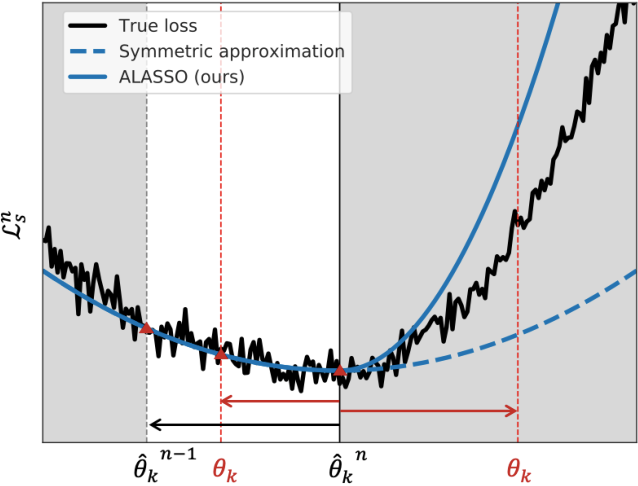
\includegraphics[width=.9\linewidth]{images/Alasso_Idea.png}
    \caption[Visualization of ALASSO]{Illustration of the ALASSO idea taken from the paper \cite{park2019continual}. The authors of ALASSO state that, SI underestimates the 
    unobserved side of the loss function and hence a better approximation of the loss function is achieved by overestimating it.}
    \label{fig:Alasso}
\end{figure}
%TODO: Include image of Alasso idea in here

\subsubsection{IMM}
Incremental Moment Matching (IMM) is a structural regularization approach to prevent catastrophic forgetting, proposed by Lee et al. \cite{lee2017overcoming}.
IMM deviates from approaches like MAS and EWC in that it should not be seen as a single method but rather a framework of multiple methods, many of which can be
combined with each other. The main idea of IMM is to match the first and second moments of the posterior distribution $p(\theta \mid D_{1:N})$ of the model 
parameters given all tasks up to the current one. As in EWC, the posterior distribution cannot be computed, it is approximated via a Gaussian distribution which
we call $q_{1:N}$. The first approach to matching these moments is called \textbf{Mean-based Incremental Moment Matching}, also known as mean-IMM. The weight
update of mean-IMM is the analytical solution of the problem to minimize the weighted sum of Kullback-Leibler (KL) divergences between each $q_i$ and $q_{1:N}$
\cite{goldberger2004hierarchical}, i.e. the solution to
\begin{equation}
    \argmin_{\mu^*_{1:N},\Sigma^*_{1:N}} \sum_{i=N-k}^N \alpha_i \cdot KL(q_i \mid \mid q_{1:N})
\end{equation}
which is given by
\begin{gather}
    \mu^*_{1:N} = \sum_{i=N-k}^N \alpha_i \cdot \mu_i \\
    \Sigma^*_{1:N} = \sum_{i=N-k}^N \alpha_i (\Sigma_i + (\mu_i - \mu^*_{1:N})(\mu_i - \mu^*_{1:N})^T)
\end{gather}
The $\alpha_i$ here are the mixing coefficents which weigh the previousl $k$ tasks and have the constraint $\sum_{i=N-k}^N \alpha_i = 1$.  \\
The second approach to matching the moments is called \textbf{Mode-based Incremental Moment Matching}, and it is also known as mode-IMM. mode-IMM
further incorporates covariance information from previous tasks to better match the first and second moments of the posterior distribution. 
The mean and covariance update for mode-IMM is given by
\begin{gather}
    \mu^*_{1:N} = \sum_{i=N-k}^N \alpha_i \cdot (\sum_{i=N-k}^N \alpha_i \Sigma_i^{-1} \mu_i) \\
    \Sigma^*_{1:N} = (\sum_{i=N-k}^N \alpha_i  \Sigma_i^{-1})^{-1}
\end{gather}
To approximate the covariance matrix, mode-IMM uses the inverse of the Fisher Information Matrix like EWC. Furthermore, the authors assume that
the model parameters are pairwise independent, making the covariance matrix diagonal and therefore saving a lot of computation. \\ 
Apart from moment matching methods, IMM also includes approaches to transfer model parameters from previous tasks. The first approach is called
\textbf{Weight Transfer}. When using continual learning with Weight Transfer the model parameters of the previous task are used as initialization for the
current task. This approach is very similar to the term Warm Start commonly used in Active Learning. \textbf{L2-transfer} is the next transfer technique
which is a special form of L2-regularization. L2-transfer can be seen as a special form of EWC where all the $F_i$s are set to 1. With L2 transfer the loss
function is altered to 
\begin{equation}
    \log p(y_N \mid X_N, \mu_N) - \lambda \cdot {\lVert \mu_N - \mu_{N-1} \rVert}^2_2
\end{equation}
with $\lambda$ being a hyperparameter. The third transfer technique is \textbf{Drop-transfer}. Drop-transfer
\begin{equation}
    \hat{\mu}_{N,i} = \begin{cases} \mu_{N,i}, & \text{if the }i \text{th node is turned off} \\
    \frac{1}{1-p} \cdot \mu_{N,i} - \frac{p}{1-p} \cdot \mu_{N-1,i}, & \text{otherwise}  \end{cases}
\end{equation}
where $p$ is the dropout ratio. Dropout-transfer can be seen as a further regularizer for continual learning, with similar effect to L2-transfer albeit
being orthogonal to it.
\begin{algorithm}
    \caption{IMM with weight-transfer, L2-transfer} \label{alg:IMM}
    \begin{algorithmic}
        \Require data $f\{ (X_1,Y_1),\ldots,(X_N,Y_N)\}$, balancing hyperparameter $\alpha$ with $\sum_{i=1}^k \alpha_i = 1$,
        regularization hyperparameter $\lambda$
        \return $w_{1:N}$
        \State $w_0 \leftarrow $ InitializeNN()
        \For{$i=1:N$}
            \State $w_{i*} \leftarrow w_{i-1}$
            \State Train($w_{i*},X_i,Y_i$) with $L(w_{i*},X_i,Y_i) + \lambda \cdot (\lVert w_{i*} - w_{i-1} \rVert)^2_2$
            \State $m=\max (0,i-k)$
            \If{type is mean-IMM}
            \State $w_{i*} \leftarrow \sum_{t=max(0,i-k)}^i \alpha_t w_{t}$
            \ElsIf{type is mode-IMM}
            \State $F_{i*} \leftarrow$ CalculateFisherMatrix($w_{i*},X_i,Y_i$)
            \State $\Sigma_{1:i} \leftarrow (\sum_{t=max(0,i-k)}^i \alpha_t F_{t*} w_{t*})^{-1}$
            \State $w_{i*} \leftarrow \Sigma_{1:i} \cdot (\sum_{t=max(0,i-k)}^i \alpha_t F_{t*} w_{t*})$
            \EndIf
        \EndFor
    \end{algorithmic}
\end{algorithm}
% Structure: First some general introduction then present
% the different approaches used in the experiments (EWC, MAS, ALASSO, IMM, potentially Replay?)


\section{Model Stealing}
\label{sec:Related_work:Model_Stealing}
% Hier Active Thief erwähnen und falls später noch defense strategies verwendet werden das ebenfalls noch erwähnen

\subsection{Knockoff Nets}
\label{sec:Related_work:Model_Stealing:Knockoff_Nets}
Knockoff Nets was published by Orekondy et al. \cite{orekondy2019knockoff}, and it was the first approach which focused only on stealing the functionality
of the model instead of inferring hyperparameters, model architecture etc. Orekondy et al. used a variety of substitute models, thief datasets and query
selection strategies to empirically evaluate how these factors influence the model stealing process. More precisely, they test the substitute models
Alexnet \cite{krizhevsky2017imagenet}, Resnet, VGG and Densenet \cite{huang2017densely} using Caltech-256,CUBS-200-2011, Indoor-Scenes, Diabetic-Retinopathy,
ILSVRC and OpenImages as thief datasets as well as a random query selection strategy and a reinforcement learning approach. Orekondy et al. make the following
key findings: 
\begin{itemize}
    \item The choice of substitute model has a negligible impact on the overall success of the model stealing attack. Nevertheless, it is advised to use a
    substitute model with a rather complex architecture.
    \item Randomly querying the target model with images from the thief dataset yields remarkably good results. It should be noted however, that the reinforcement
    learning approach used by Orekondy et al. is able to achieve comparable accuracies with significantly less data points, depending on the dataset.
    \item There is a direct correlation between the top-$k$ outputs generated by the target model and the maximum achievable accuracy of the model stealing attack.
    In other words, more information about the prediction output directly leads to better results.
\end{itemize}
\subsection{ActiveThief}
\label{sec:Related_work:Model_Stealing:ActiveThief}
ActiveThief is a novel model stealing approach proposed by Pal et al. \cite{pal2020activethief}. Inspired by prior theoretical \cite{chandrasekaran2020exploring}
and practical work \cite{shi2018active}, they use Active Learning to choose which samples to query the target model. Using Active Learning in the model stealing
domain comes with three major benefits: First, it makes it easier for the attacker to create a thief dataset. Data is abundant nowadays while labeling large amounts
of data to this day is a time-intensive task. By using Active Learning, which works on unlabeled data, the process of creating a thief dataset is sped up immensely.
Second, Active Learning aims to query the most informative samples, yielding the most performant model with as little data as possible. Third, by using samples selected
by Active Learning to query the target model, the model stealing attack can successfully be disguised as a benign query process. Pal et al. demonstrate this by showing 
that ActiveThief successfully evades PRADA \cite{juuti2019prada}, a state-of-the-art model stealing defense which detects attacks by analyzing the distribution of distances
between queries. \\
The authors of ActiveThief evaluate their framework using the Active Learning strategies Random, Uncertainty \cite{lewis1994sequential}, CoreSet \cite{sener2017active},
DeepFool-based Active Learning (DFAL) \cite{ducoffe2018adversarial} and a custom combination of DFAL and CoreSet. They use a custom CNN architecture for both target and
substitute model and show that ActiveThief is able to successfully steal the target model for multiple benchmark datasets such as MNIST and CIFAR-10. A visualization of
the model stealing workflow proposed by Pal et al. is shown in Figure \ref{fig:ActiveThief}.

\begin{figure} [ht]
    \centering
    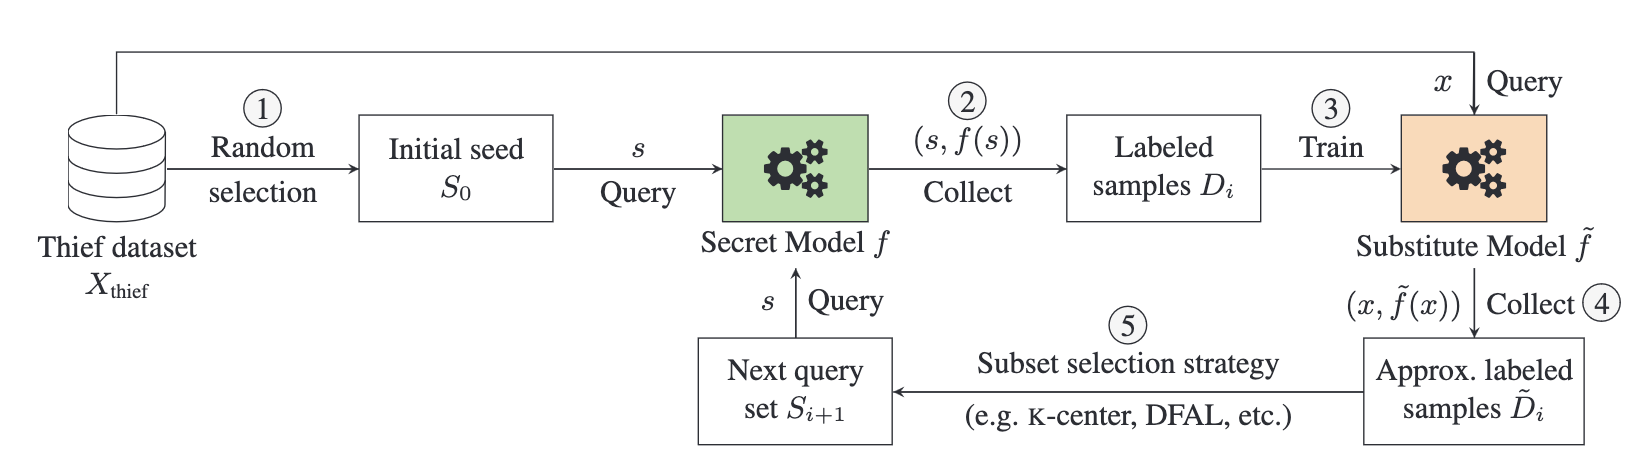
\includegraphics[width=.9\linewidth]{images/ActiveThief_Idea.png}
    \caption[Visualization of ActiveThief]{Illustration of the model stealing workflow proposed by \cite{pal2020activethief}. Inspired by
    \cite{chandrasekaran2020exploring}, Pal et al. use active learning to select the next samples to query the target model.}
    \label{fig:ActiveThief}
\end{figure}

\dots
%% ---------------------
%% | / Example content |
%% ---------------------